%%%%%%%%%%%%%%%%%%%%%%%%%%%%%%%%%%%%%%%%%%%%%%%%%%%%%%%%%%
%
% WARNING : use common_nnet.tex
%
%%%%%%%%%%%%%%%%%%%%%%%%%%%%%%%%%%%%%%%%%%%%%%%%%%%%%%%%%%


%the different layers in our deep network are learning at vastly different speeds. In particular, when later layers in the network are learning well, early layers often get stuck during training, learning almost nothing at all.
%there's an intrinsic instability associated to learning by gradient descent in deep, many-layer neural networks. This instability tends to result in either the early or the later layers getting stuck during training
\begin{frame}{Experimental observations (MNIST task) - 1}
  \begin{block}{The MNIST database}
    \includegraphics[width=0.6\textwidth]{../figs/mnist}
  \end{block}
  \begin{block}{Comparison of different depth for feed-forward architecture}
     \begin{center}
       \resizebox{0.8\columnwidth}{!}{
         \begin{tabular}[h]{lclclclclcl}
          \color{red}\inp\lid{1} & & \inp\lid{2}  && \inp\lid{3} & &\inp\lid{L} \\
          \color{red}\layer &\connection &\layer &\connection &\layer &\dotted &\layer &\connection &\color{red}\layer \\[-2ex]
          & \raisebox{\raiseW}{\W\lid{1}} &\outp\lid{1}   &\raisebox{\raiseW}{\W\lid{2}} &\outp\lid{2}  &&\outp\lid{L-1}&\raisebox{\raiseW}{\W\lid{L}} &\color{red}\outp\lid{L}: output 
        \end{tabular}
      }
      \begin{itemize}
      \item Hidden layers have a sigmoid activation function.
      \item The output layer is a softmax.
      \end{itemize}
  \end{center}
  \end{block}
\end{frame}

\begin{frame}{Experimental observations (MNIST task) - 2}
  \begin{block}{Varying the depth}
    \begin{itemize}
    \item Without hidden layer:  $\approx 88\%$ accuracy
    \item 1 hidden layer (30): $\approx 96.5\%$ accuracy
    \item 2 hidden layers (30): $\approx 96.9\%$ accuracy
    \item 3 hidden layers (30): $\approx 96.5\%$ accuracy
    \item 4 hidden layers (30): $\approx 96.5\%$ accuracy
    \end{itemize}
  \end{block}\pause
  \begin{columns}
    \begin{column}{0.5\textwidth}
      \includegraphics[width=1\textwidth]{../figs/training_speed_4_layers}
    \end{column}
    \begin{column}{0.5\textwidth}
      \scriptsize (From \url{http://neuralnetworksanddeeplearning.com/chap5.html})
    \end{column}
  \end{columns}
\end{frame}


\begin{frame}{Intuitive explanation}
  Let consider the simplest deep neural network, with just a single neuron in each layer.
  \begin{center}
    \includegraphics[width=0.7\textwidth]{../figs/oneUnitNet}
  \end{center}
  $w_i, b_i$ are resp. the weight and bias of neuron $i$ and $C$ some cost function. 
  \begin{block}{Compute the gradient of $C$ \textit{w.r.t} the bias $b_1$}
    \begin{align}
      \frac{\partial C }{\partial b_1} &=       \frac{\partial C}{\partial y_4}      \times
      \frac{\partial y_4}{\partial a_4}   \times \frac{\partial a_4}{\partial y_3} \times
      \frac{\partial y_3}{\partial a_3}   \times \frac{\partial a_3}{\partial y_2} \times
      \frac{\partial y_2}{\partial a_2}   \times \frac{\partial a_2}{\partial y_1} \times
      \frac{\partial y_1}{\partial a_1}   \times \frac{\partial a_1}{\partial b_1} \\
      &=       \frac{\partial C}{\partial y_4}      \times
      \sigma'(a_4) \times w_4 \times
      \sigma'(a_3) \times w_3 \times
      \sigma'(a_2) \times w_2 \times
      \sigma'(a_1) 
    \end{align}
  \end{block}
\end{frame}

\begin{frame}{Intuitive explanation - 2}
  \begin{block}{The derivative of the activation function: $\sigma'$}
    \begin{columns}
      \begin{column}{0.5\textwidth}
%%%%%%% logistic
          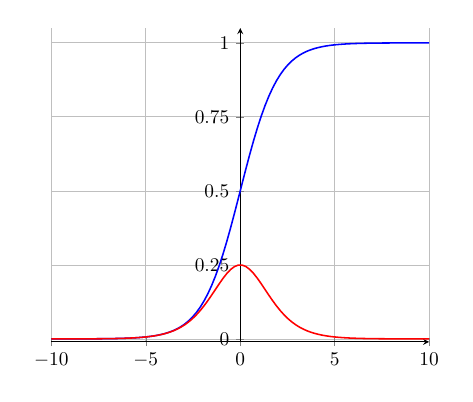
\begin{tikzpicture}[scale=0.7]
            \begin{axis}%
              [ %%%%%%%%%%%%%%%%%
              grid=major, %
              xmin=-10, % 
              xmax=10, % 
              axis x line=bottom, % 
              ytick={0,.25,.5,.75,1.0}, %
              ymax=1.05, % 
              ymin = -0.01, %
              axis y line=middle, % 
              every  axis y label/.style={at={(current axis.north
                  west)},above=2mm} ]% 
              \addplot%
              [ blue,thick,%
              mark=none, samples=100, domain=-10:10, ]
              (x,{ (1/(1+exp(-x))) });
              \addplot%
              [ red,thick,%
              mark=none, samples=100, domain=-10:10, ]
              (x,{ (1/(1+exp(-x)))*(1-(1/(1+exp(-x)))) });
            \end{axis}
          \end{tikzpicture}
      \end{column}
      \begin{column}{0.5\textwidth}
        $$
        \sigma'(x) = \sigma(x)(1-\sigma(x))
        $$
        But weights are initialize around $0$. 
      \end{column}
    \end{columns}
  \end{block}
  \important{The different layers in our deep network are learning at vastly different speeds:}
  \begin{itemize}
  \item when later layers in the network are
    learning well,
  \item early layers often get stuck during training,
    learning almost nothing at all.
\end{itemize}
\end{frame}

\begin{frame}{A first Solution}
  \begin{block}{Change the activation function (Rectified Linear Unit or
      ReLU)}
    \begin{columns}
      %%%%%%%%% relu
      \begin{column}{0.4\textwidth}
        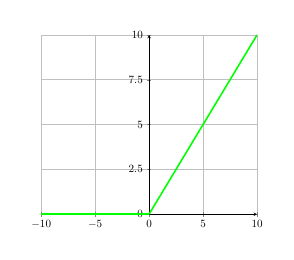
\begin{tikzpicture}[scale=0.4]
          \begin{axis}%
            [ %%%%%%%%%%%%%%%%%
            grid=major, %
            xmin=-10, % 
            xmax=10, % 
            axis x line=bottom, % 
            ytick={0,2.5,5,7.5,10}, %
            ymax=10, % 
            ymin = -0.01, %
            axis y line=middle, % 
            every  axis y label/.style={at={(current axis.north
                west)},above=2mm} ]%
            \addplot%
            [ green,line width=0.5mm,%
            mark=none, samples=100, domain=0:-10, ]
            (x,{0.00});
            \addplot%
            [ green,line width=0.5mm,%
            mark=none, samples=100, domain=0:10, ]
            (x,x);
          \end{axis}
        \end{tikzpicture}
      \end{column}
      \begin{column}{0.6\textwidth}
        \begin{itemize}
        \item Avoid the vanishing gradient
        \item  Some units can "die''
        \end{itemize}
        See~\cite{Glorot11Rectifier} for more details
      \end{column}
    \end{columns}
  \end{block}
  \begin{block}{Variants}
    \begin{itemize}
    \item Leaky ReLU~\cite{Maas13lrelu}
    \item Soft-plus $log(1+e^x)$
    \end{itemize}
    And many more, see \url{https://pytorch.org/docs/stable/nn.html}
  \end{block}
  \begin{block}{More details}
    See~\cite{Hochreiter01Gradient,Glorot10Understanding,Lecun12Efficient} 
  \end{block}
\end{frame}


% \begin{frame}{A question}
%   Why adding a layer can lower the performance ? \pause
%   \begin{itemize}
%   \item Overfitting ? and what about the identity
%   \item Vanishing gradient ? and with the \textit{Relu} ? 
%   \end{itemize} \pause
%   \begin{block}{Residual block}
%     \begin{columns}
%     \column{0.5\textwidth}
%     From~\cite{He16Residual}
%     \begin{itemize}
%     \item Add a skip connection
%     \item The model learn the "residual"
%       $$
%       \y = \mathcal{F}(\x) = \x + \mathcal{R}(\x)
%       $$
%     \end{itemize}
%       \column{0.5\textwidth}
%       \begin{center}
%         \includegraphics[width=\textwidth]{../figs/residual}
%       \end{center}
%     \end{columns}
%     A simple version of highway networks~\cite{Srivastava15Highway}
%   \end{block}
% \end{frame}


% \begin{frame}{Residual block}
%   \begin{block}{Forward}
%     \begin{align*}
%       \y &= \mathcal{F}(\x) = \x + \mathcal{R}(\x), \textrm{ or }\\
%       \y &= \W_{s} \x + \mathcal{R}(\x), \textrm{ to adapt the dimension}
%     \end{align*}
%   \end{block}
%   \begin{block}{Backward}
%     Assume a residual block for the layer $l$ in the network. Training requires:
%     \begin{itemize}
%     \item $\frac{\partial l }{\partial\W\lid{l}}$ for the update of the layer
%     \item $\frac{\partial l }{\partial\x\lid{l}}$ for the backpropagation
%     \end{itemize}
%     \begin{align*}
%       \frac{\partial l }{\partial\x\lid{l}} &=       \frac{\partial l }{\partial\y\lid{l}} \times  \frac{\partial\y\lid{l}}{\partial\x\lid{l}}\\
%                                             &= \frac{\partial l }{\partial\y\lid{l}} \times  (1+\frac{\partial\mathcal{R}(\x\lid{l})}{\partial\x\lid{l}})
%     \end{align*}
%   \end{block}
% \end{frame}

